%\VignetteIndexEntry{geneXtendeR Vignette}
%\VignettePackage{geneXtendeR}

\documentclass[12pt]{article}

\usepackage{float}
\title{geneXtendeR}
\author{Bohdan B. Khomtchouk}

\RequirePackage{/Library/Frameworks/R.framework/Versions/3.2/Resources/library/BiocStyle/resources/tex/Bioconductor}

\AtBeginDocument{\bibliographystyle{/Library/Frameworks/R.framework/Versions/3.2/Resources/library/BiocStyle/resources/tex/unsrturl}}

\usepackage{Sweave}
\begin{document}
\Sconcordance{concordance:geneXtendeR.tex:geneXtendeR.Rnw:%
1 10 1 1 2 1 0 1 2 2 1 1 0 26 1 1 3 2 0 1 1 3 0 2 2 4 0 1 2 2 1 1 3 5 0 1 2 6 1 %
1 2 4 0 1 2 4 1 1 2 1 0 1 1 3 0 1 2 6 1 1 2 5 0 1 2 6 1 1 2 5 0 1 2 6 1 1 2 5 0 %
1 2 6 1 1 2 5 0 1 2 6 1 1 2 1 0 2 1 4 0 1 2 8 1 1 2 1 0 2 1 4 0 1 2 4 1 1 2 1 0 %
2 1 6 0 1 2 4 1 1 2 1 0 2 1 4 0 1 2 6 1 1 2 1 0 2 1 4 0 1 2 4 1 1 2 1 0 1 1 6 0 %
1 2 2 1 1 2 1 0 1 1 6 0 1 2 2 1 1 2 30 0 1 2 2 1 1 2 1 0 2 1 67 0 1 2 4 1 1 2 1 %
0 3 1 26 0 1 2 6 1 1 2 1 0 3 1 3 0 1 2 14 1 1 2 1 0 4 1 3 0 1 2 8 1 1 2 1 0 4 1 %
3 0 1 2 9 1 1 2 4 0 1 2 11 1 1 2 27 0 1 2 8 1 1 2 4 0 1 2 10 1 1 2 4 0 1 2 14 1 %
2 2 16 1 1 2 5 0 1 2 5 1 1 2 4 0 1 2 6 1 1 2 1 0 5 1 74 0 1 3 61 1}


\maketitle

\begin{figure}[H]
\centering

\includegraphics[width=50mm,scale=0.5]{figures/geneXtendeRlogo.png}
\end{figure}

\texttt{geneXtendeR} is designed to optimally annotate a histone modification ChIP-seq peak input file with functionally important genomic features (e.g., genes associated with peaks) based on optimization calculations.  These optimization calculations automatically factor in experimental conditions such as the broadness of the histone peaks found in the specific tissue of the ChIP-seq peak file.  

To accomplish this level of custom-tailored data-centric analysis, \texttt{geneXtendeR} first optimally extends the boundaries of every gene in a genome by some genomic distance (in DNA base pairs) for the purpose of flexibly incorporating cis-regulatory elements, such as enhancers and promoters, as well as downstream elements that are important to the function of the gene relative to an epigenetic histone modification ChIP-seq dataset.  This action effectively transforms genes into ``gene-spheres", a new term that we coin to emphasize the 3D-nature of heterochromatin.  A gene-sphere is composed of cis-regulatory elements (e.g., proximal promoters +/- $\approx 3$ kb from TSS), distal regulatory elements (e.g., enhancers), transcription start/end sites (TSS/TES), exons, introns, and downstream elements of a gene.  As such, \texttt{geneXtendeR} maximizes the signal-to-noise ratio of locating gene regions closest to and directly under peaks. By performing a computational expansion of this nature, ChIP-seq reads that would initially not map strictly to a specific gene can now be optimally mapped to the regulatory regions of the gene, thereby implicating the gene as a potential candidate, and thereby making the ChIP-seq experiment more successful. Such an approach becomes particularly important when working with epigenetic histone modifications that have inherently broad peaks with a diffuse range of signal enrichment (e.g., H3K9me1, H3K27me3). 

A series of diagnostic criteria are used to compute optimal gene extensions tailored to the tissue-specific broadness of the specific epigenetic mark in the ChIP-seq peak input file:

First, install the \texttt{geneXtendeR} R package via \texttt{install.packages("geneXtendeR")} and load it in:

\begin{Schunk}
\begin{Sinput}
> library(geneXtendeR)
\end{Sinput}
\end{Schunk}

Then loads the \texttt{rtracklayer} R package, which contains the \texttt{readGFF()} command used to retrieve gene transfer format files of any model organism (discussed further below).

\texttt{geneXtendeR} also requires the installation of an external program called \texttt{bedtools}.  This program must be pre-installed on your computer prior to using \texttt{geneXtendeR}.  As described in the \texttt{README} file found in the top-level directory of this \texttt{geneXtendeR} R package, detailed installation instructions can be accessed here: \url{http://bedtools.readthedocs.io/en/latest/content/installation.html}.  You may follow this recipe in a Terminal:

\begin{figure}[H]
\centering
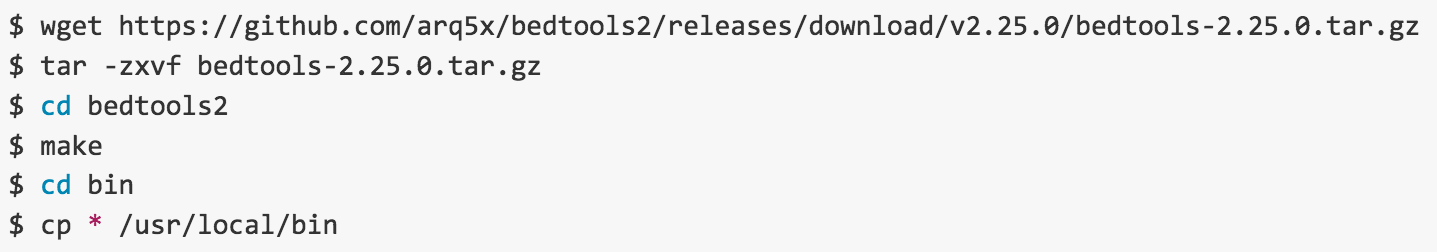
\includegraphics{figures/bedtoolsInstallation.png}
\end{figure}

After \texttt{bedtools} has been installed, the \texttt{geneXtendeR} package is fully configured and setup for use. 

First, load in a GTF file into your R environment, e.g.:

\begin{Schunk}
\begin{Sinput}
> rat <- readGFF("ftp://ftp.ensembl.org/pub/release-84/gtf/
+                       rattus_norvegicus/Rattus_norvegicus.Rnor_6.0.84.gtf.gz")
\end{Sinput}
\end{Schunk}

URLs may be obtained as direct links from: \url{http://useast.ensembl.org/info/data/ftp/index.html}.  Click on the ``GTF" link under the ``Gene sets" column for a particular species and then right-click (or command-click on Mac OS X) the name of the file containing the species name/version number and file extension .gtf.gz (e.g., Homo\_sapiens.GRCh38.84.gtf.gz, Mus\_musculus.GRCm38.84.gtf.gz, etc), and select ``Copy Link Address".  Then, paste it into the \texttt{readGFF()} as shown above.  This will create an R data frame object containing the respective gene transfer format file.

Next, use this R object to create a series of \texttt{geneXtendeR} files at some user-specified interval:

\begin{Schunk}
\begin{Sinput}
> generate(rat, 0, 10000, 500)
\end{Sinput}
\end{Schunk}


This command generates 21 individual whole-genome files: 0, 500, 1000, ..., and 10000 bp upstream extension files for the rat (\emph{Rattus norvegicus}) genome, each having an automatic 500 bp downstream extension.

Next, the user must input their peak data from some peak caller (e.g., SICER, MACS2, etc).  The peak data must contain only three tab-delimited columns: chromosome number, peak start, and peak end.  See \texttt{?samplepeaksinput} for an example.  Once the peak input data (e.g., ``myfilename.txt") has been assembled properly, it must be properly formatted prior to the execution of various geneXtendeR analyses:

\begin{Schunk}
\begin{Sinput}
> peaksInput("myfilename.txt")
\end{Sinput}
\end{Schunk}

This command properly formats the user's peak file in preparation for subsequent analyses, producing a resultant ``peaks.txt" file used in the subsequent analysis.

First, a raw count of the number of peaks that are sitting on top of a gene is calculated for each file.

\begin{Schunk}
\begin{Sinput}
> barChart()
\end{Sinput}
\end{Schunk}

\begin{figure}[H]
\centering
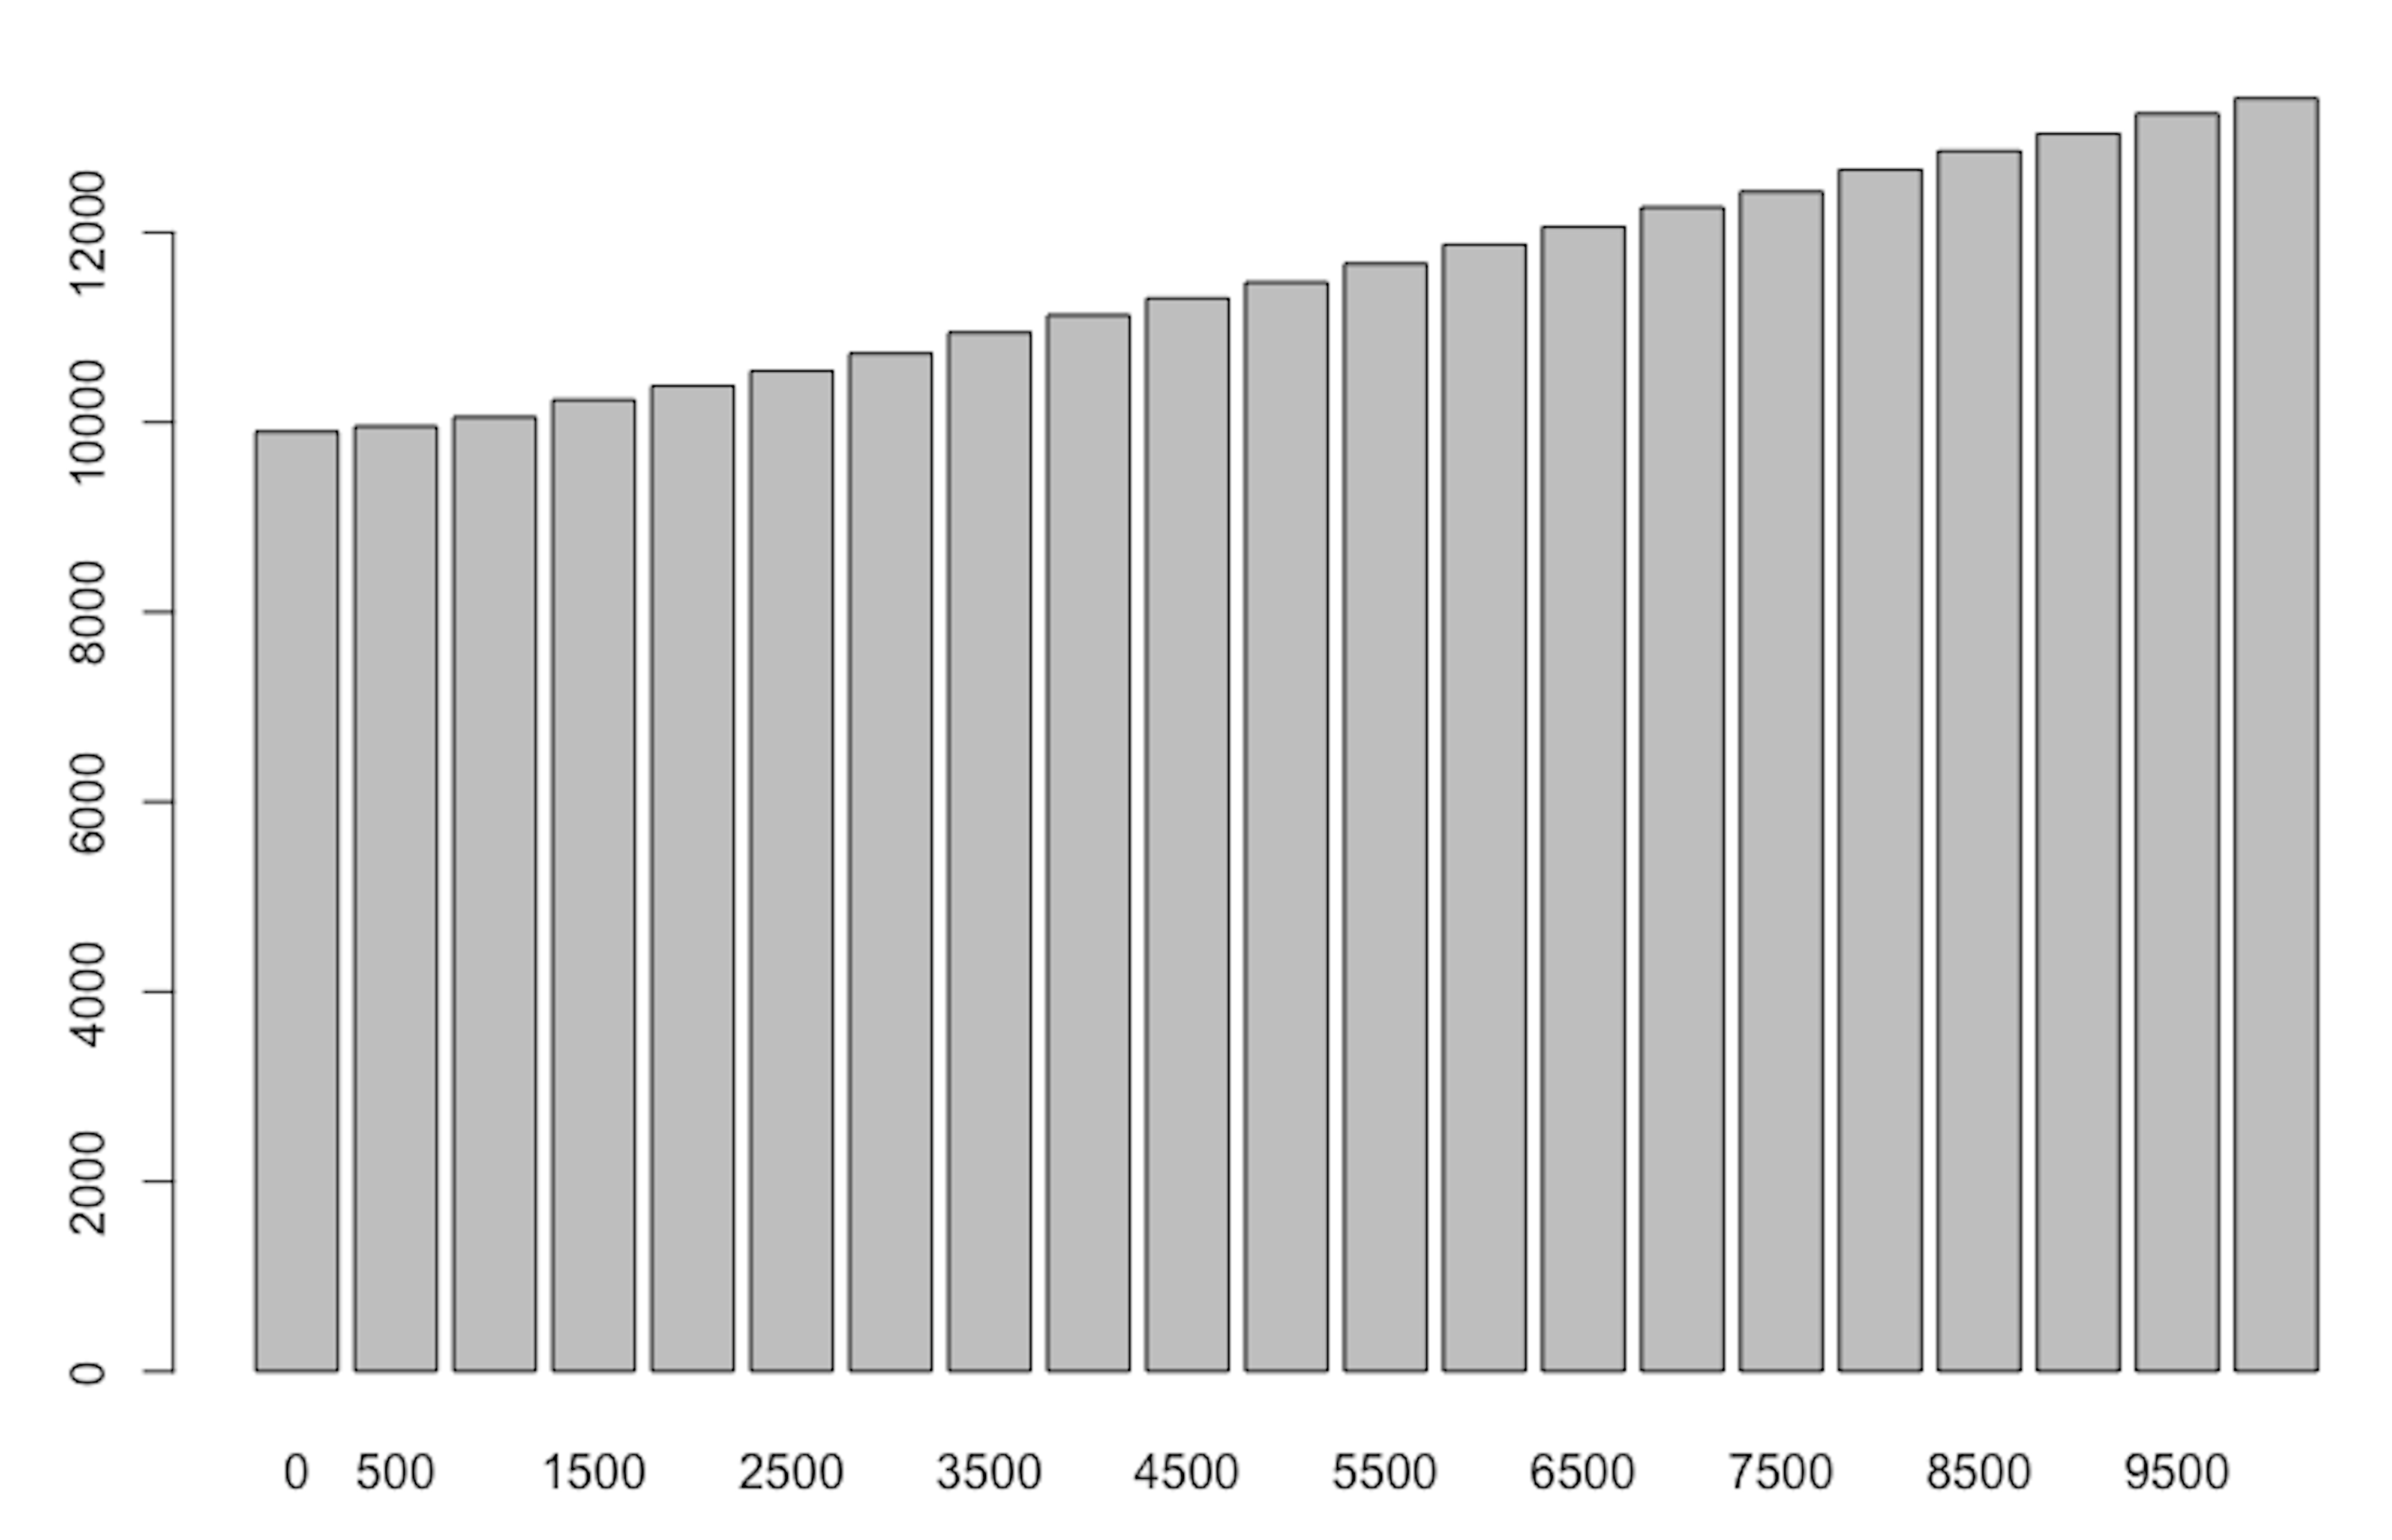
\includegraphics{figures/fig1.png}
\end{figure}

Clearly, the wider the gene-sphere, the more peaks-on-top-of-genes are found throughout the genome.  However, the law of diminishing returns begins to kick in at increasing upstream extension levels (see \texttt{linePlot()} for a visual representation):

\begin{Schunk}
\begin{Sinput}
> linePlot()
\end{Sinput}
\end{Schunk}

\begin{figure}[H]
\centering
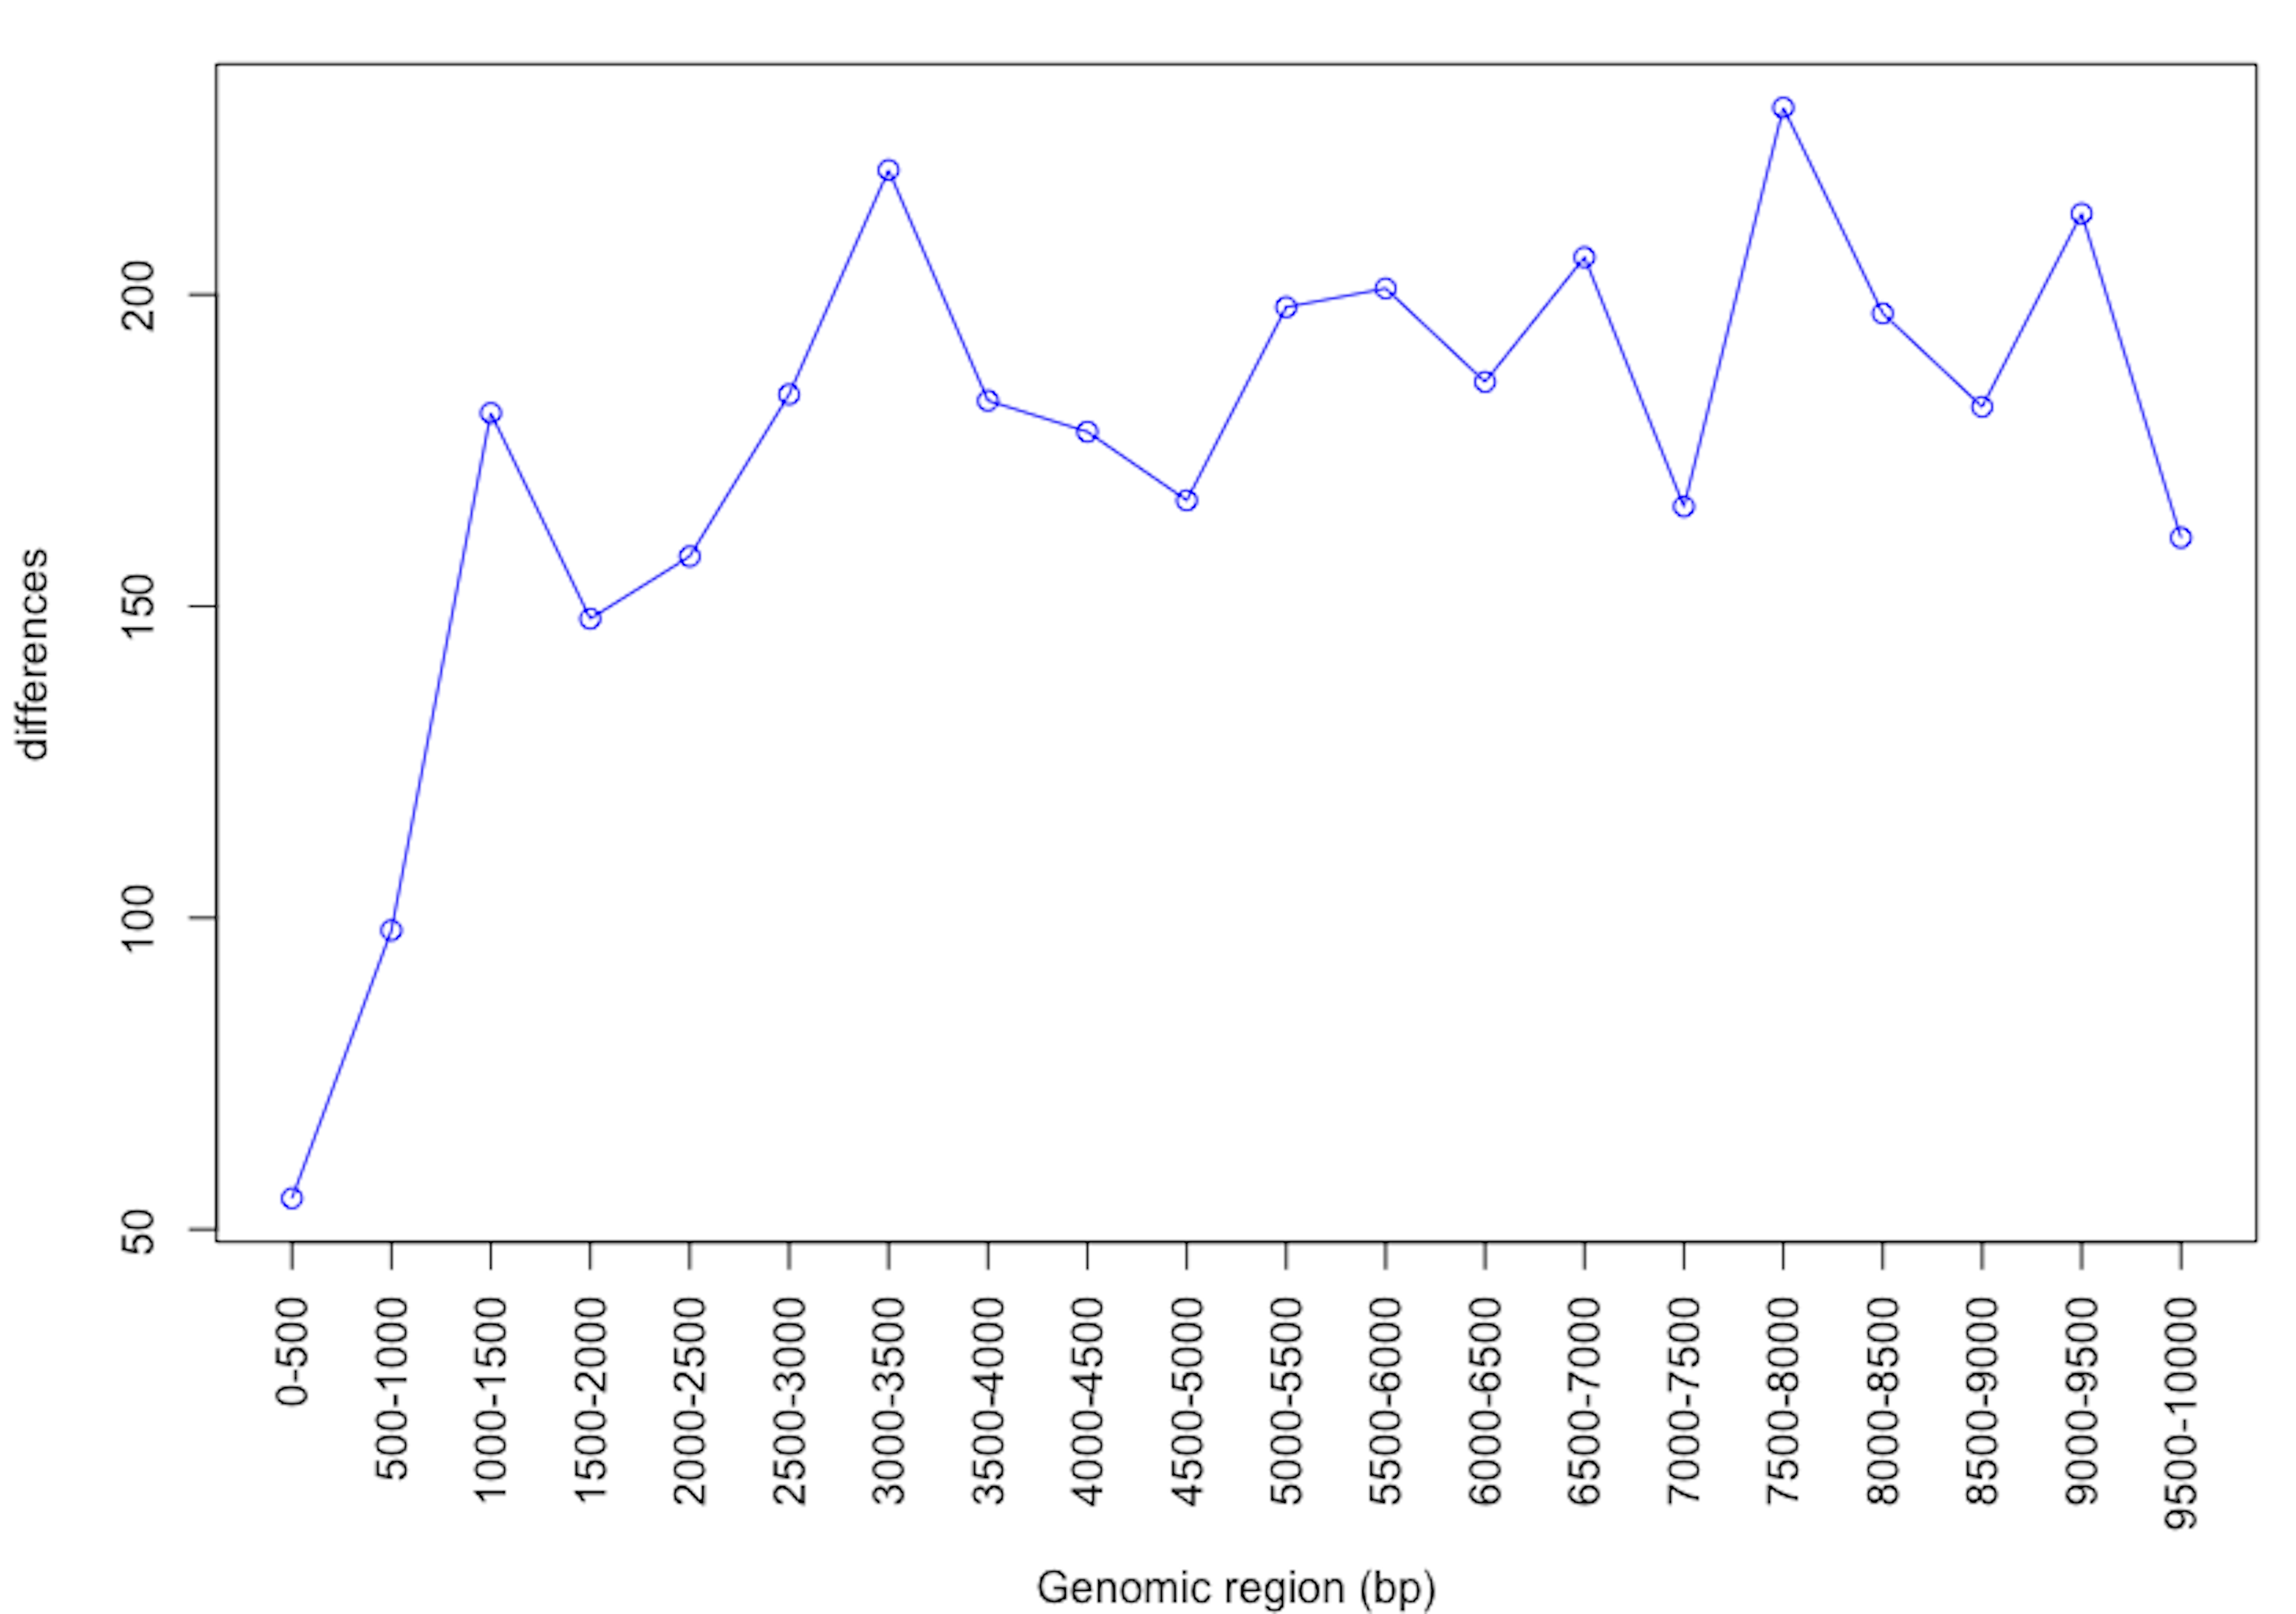
\includegraphics{figures/fig2.png}
\end{figure}

Clearly, there is a sharp rise in the number of peaks-on-top-of-genes from a 0 bp upstream extension to a 1500 bp upstream extension, and from a 2000 bp upstream extension to a 3500 bp upstream extension.  This steady rise up until 3500 bp is followed by a steady decline at subsequent extension levels followed by some noisy fluctuations.  It may be interesting to investigate what is going on in the interval from 3000 bp to 3500 bp: 

\begin{Schunk}
\begin{Sinput}
> generate(rat, 3000, 3500, 50)
> linePlot()
\end{Sinput}
\end{Schunk}

\begin{figure}[H]
\centering
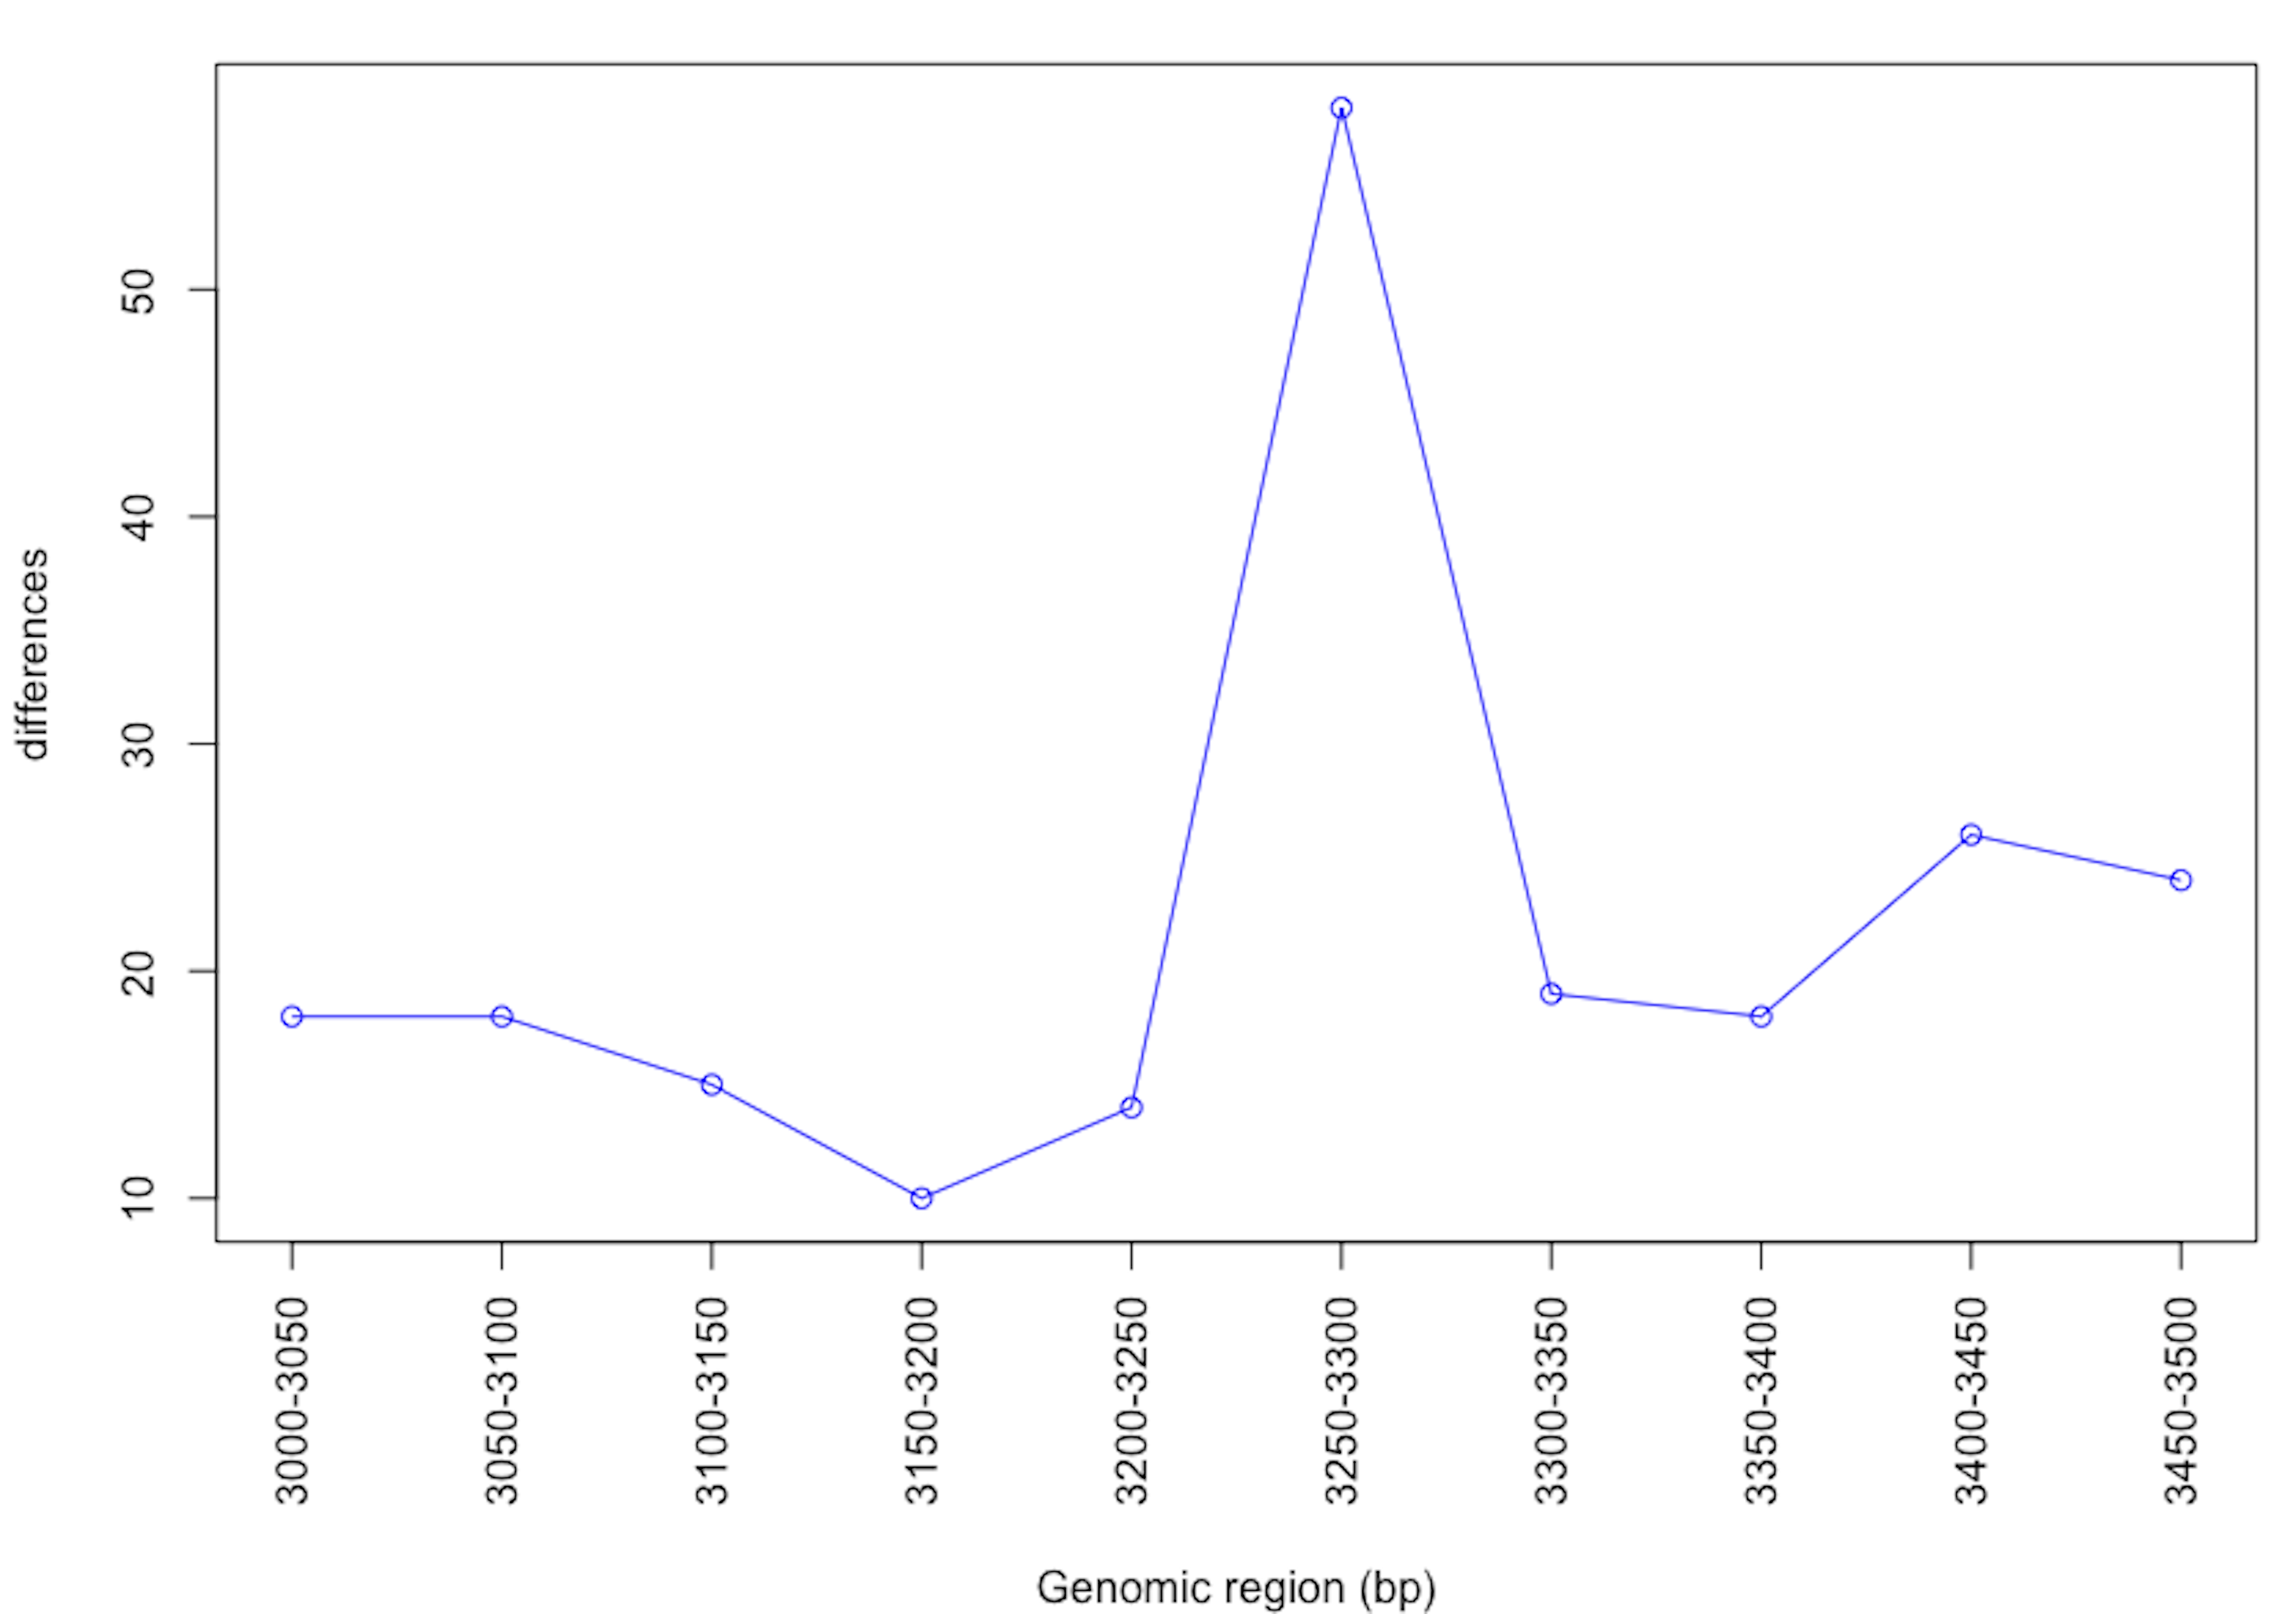
\includegraphics{figures/fig3.png}
\end{figure}

Clearly, there is a relatively sharp spike in the number of peaks-on-top-of-genes at the 3300 bp upstream extension (as compared to the 3250 bp extension).  This spike then drops back down and stays approximately constant at subsequent extension levels, exhibiting fluctuating behavior characteristic of biological noise.  

It is also possible to identify the genes that are unique amongst the 3250 and 3300 bp upstream extension levels:

\begin{Schunk}
\begin{Sinput}
> head(distinct(rat, 3250, 3300))
\end{Sinput}
\end{Schunk}

\begin{figure}[H]
\centering
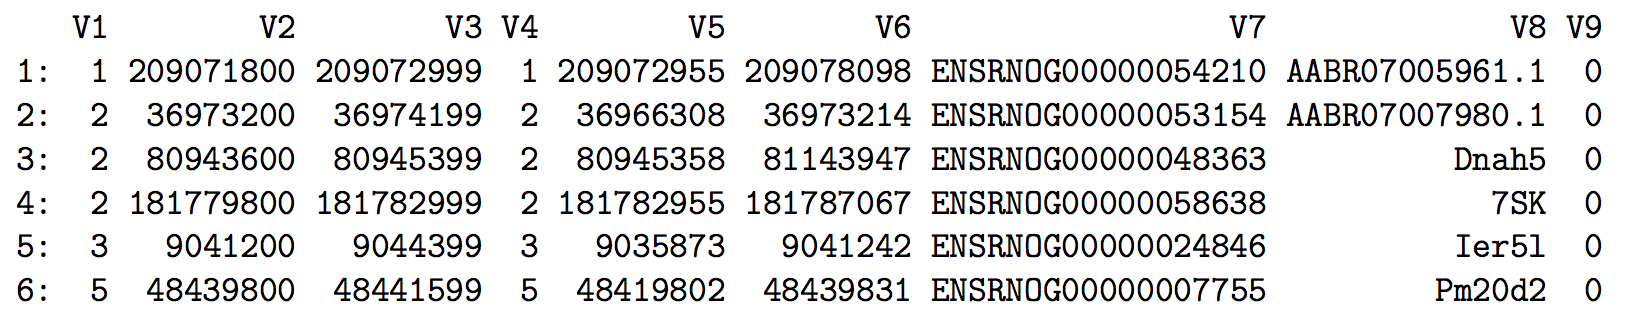
\includegraphics{figures/table1.png}
\end{figure}

shows the first six entries sorted by chromosome and start position.  \texttt{V1-V3} denote the chromosome/start/end positions of the peaks, \texttt{V4-V6} denote the respective values for the genes, \texttt{V7} is the gene ID (e.g., Ensembl ID), \texttt{V8} is the gene name, and \texttt{V9} is the distance of each respective peak to its nearest gene.  It should be noted that the X chromosome is designated by the integer 100, the Y chromosome by the integer 200, and the mitochondrial chromosome by the integer 300.  This is done for sorting purposes (see \texttt{?peaksInput} for details).  In short, the \texttt{distinct()} command finds what peaks-on-top-of-genes would be missed if a 3250 bp upstream extension is used instead of a 3300 bp extension.  Of course, subsequent follow-up extensions naturally incorporate additional peaks-on-top-of-genes, since the concept of a gene is being expanded into an ever-widening gene-sphere.  

However, even though these dynamics are to be expected, such extensions are unlikely to add significant value to the annotation of the peak file.  Taking the example of the 0-10000 bp line plot, an upstream extension beyond 3500 bp globally across every gene in a genome would most likely not accurately reflect the biology of the peak input file (since such large global upstream extensions are likely to reach considerably beyond known proximal promoter elements, especially for relatively narrow histone marks).  Such assumptions may be validated directly by the user by investigating the p-value and FDR of specific peaks using a combination of HT-seq (to count the reads) and edgeR/DESeq (to assess statistical significance).  As such, geneXtendeR is designed to be used as part of a biological workflow involving subsequent statistical analysis:

\begin{figure}[H]
\centering
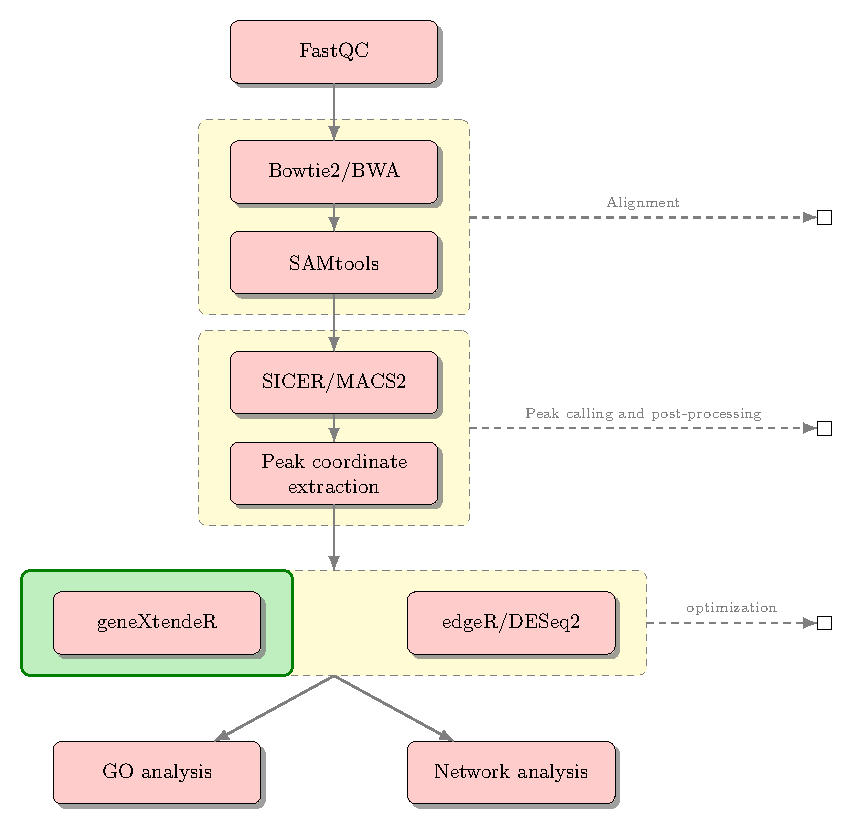
\includegraphics{figures/workflow.pdf}
\caption{Sample biological workflow using geneXtendeR in combination with existing statistical software to analyze peak significance.  Subsequent gene ontology or network analysis may be conducted on genes associated with statistically significant peaks.}
\end{figure}

It is entirely possible (and probable) for significant peaks to be present at relatively high upstream extension levels (i.e., large gene-spheres), albeit these significant peaks may be associated with biology not directly relevant to the study at-hand, due mainly to the sheer magnitude of the distance of the peak from traditional gene boundaries (where traditional gene boundaries are defined as +/- $\approx 3$ kb from TSS and +/- $\approx 0.5$kb from TES).  Consequently, it is normal for peaks-on-top-of-genes to exhibit higher levels of noise at higher upstream extension levels.  However, this does not mean that potential enhancer activity should be discounted.  For instance, it is not uncommon to see a steady rise or even a surge in the number of peaks-on-top-of-genes at higher upstream extension levels:

\begin{Schunk}
\begin{Sinput}
> generate(rat, 7000, 8500, 100)
> linePlot()
\end{Sinput}
\end{Schunk}

\begin{figure}[H]
\centering
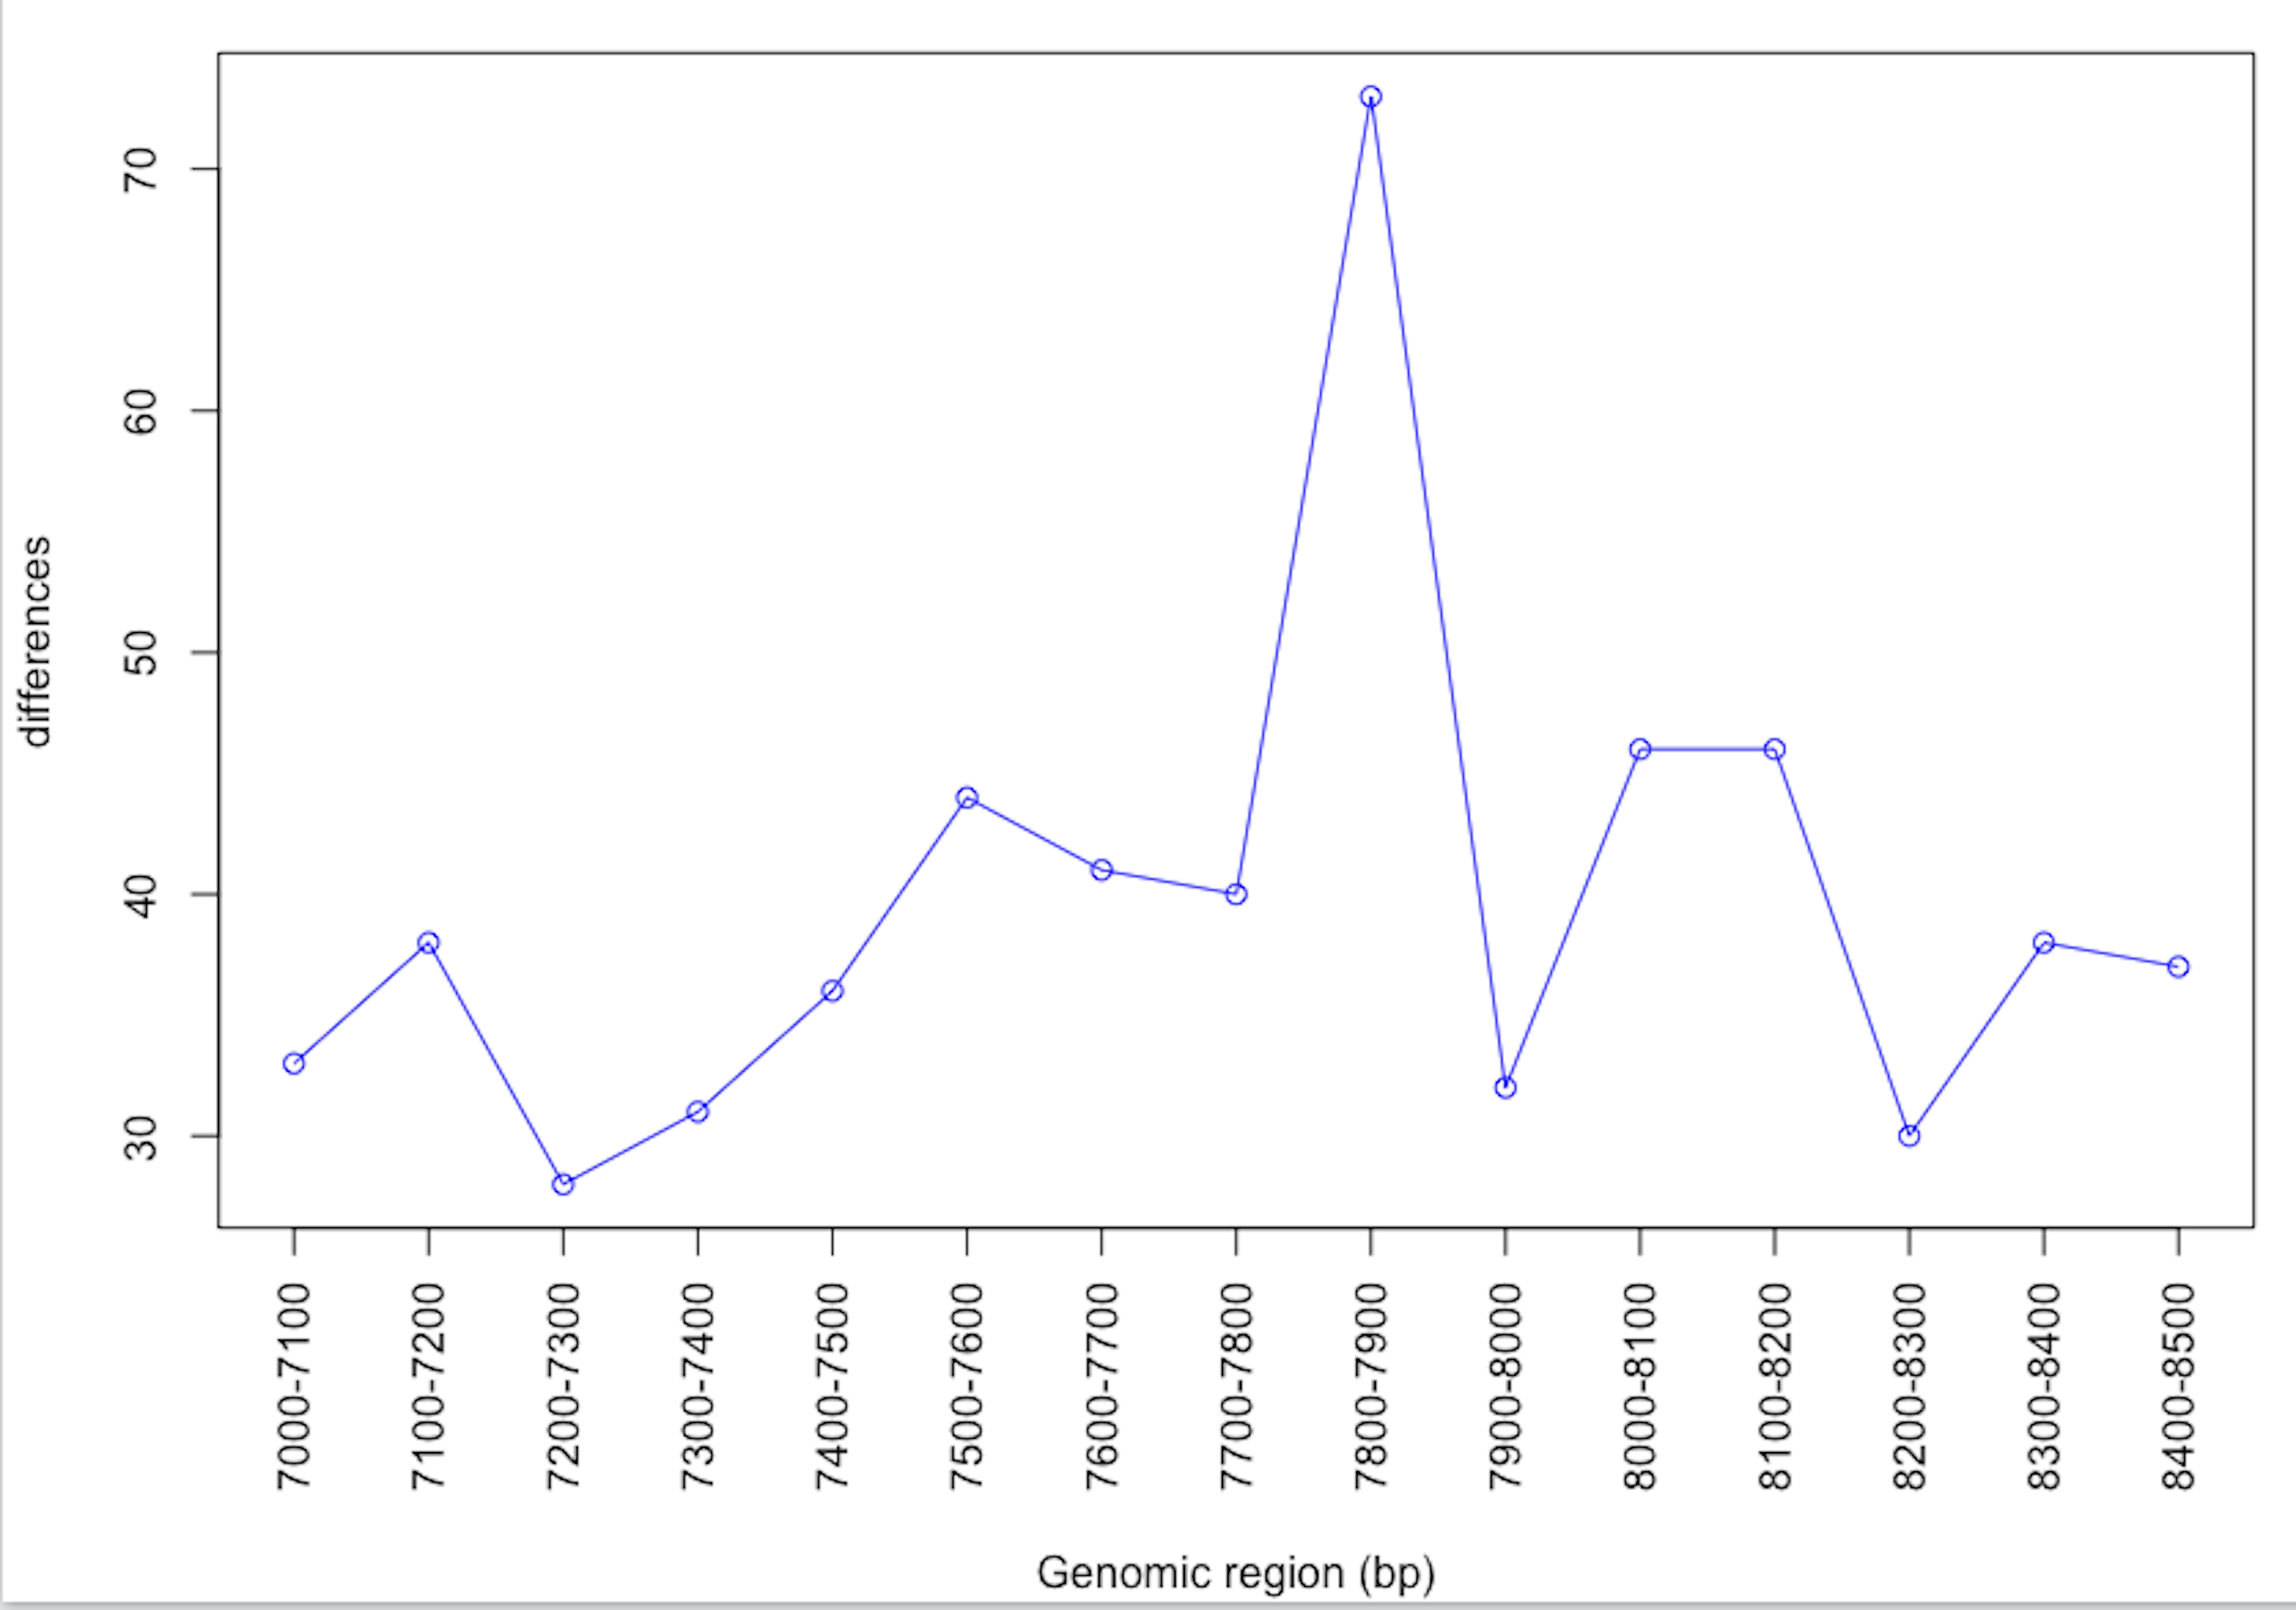
\includegraphics{figures/fig4.png}
\end{figure}

In far-out cases like this, it is particularly recommended to examine the statistical significance of peaks to get a sense for the possibility of potential enhancer activity.  Of course, such computational findings would require experimental follow-up and/or database mining for known motifs.  

Assessment of such statistical significance values is beyond the scope of geneXtendeR, in order to allow the user freedom to choose the respective statistical package/technique.  As before, first use the \texttt{distinct()} command to create a table of unique genes located under peaks between the two upstream extension levels:

\begin{Schunk}
\begin{Sinput}
> head(distinct(rat, 7800, 7900))
\end{Sinput}
\end{Schunk}

\begin{figure}[H]
\centering
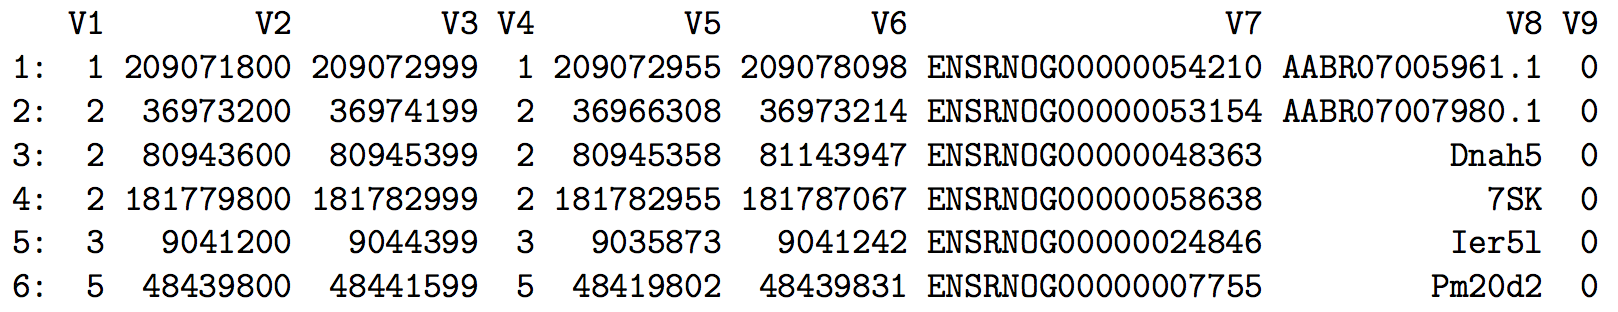
\includegraphics{figures/table2.png}
\end{figure}

Then, assess the statistical significance of these peaks using a combination of HT-seq and edgeR, or HT-seq and DESeq2, or some other appropriate combination of existing software tools.  Genes associated with the resultant statistically significant peaks may then be further assessed with gene ontology analysis or network analysis to help answer a variety of interesting research questions.  DNA sequences under peaks may be checked for the presence of known regulatory motifs (e.g., using TRANSFAC (Matys et al. 2006) or MEME/JASPAR (Sandelin et al. 2004, Bailey et al. 2009)), or for the presence of biological repeats (e.g., using RepeatMasker (Smit et al. 2015)). Pending a prospective GO/network analysis, functional validation may be followed up in the lab to test any potential regulatory sites or prospective enhancer elements, thereby bringing the computational analysis pipeline successfully back to the bench.  

Even though geneXtendeR is designed to compute (and analyze/display) optimal gene extensions tailored to the characteristics of a specific peak input file, geneXtendeR will not explicitly impose on the user the optimal extension to use, since this information is highly study-dependent and, as such, is ultimately reserved to the user's discretion.  For example, a user may choose a conservatively lower upstream extension (e.g., for studies investigating narrow peaks such as H3K4me3 or H3K9ac that exhibit a compact and localized enrichment pattern, where high upstream extensions may lose biological meaning).  An example of such user-driven decisions would be the selection of a 1500 bp upstream extension instead of a 3500 bp extension in situations like this:

\begin{figure}[H]
\centering
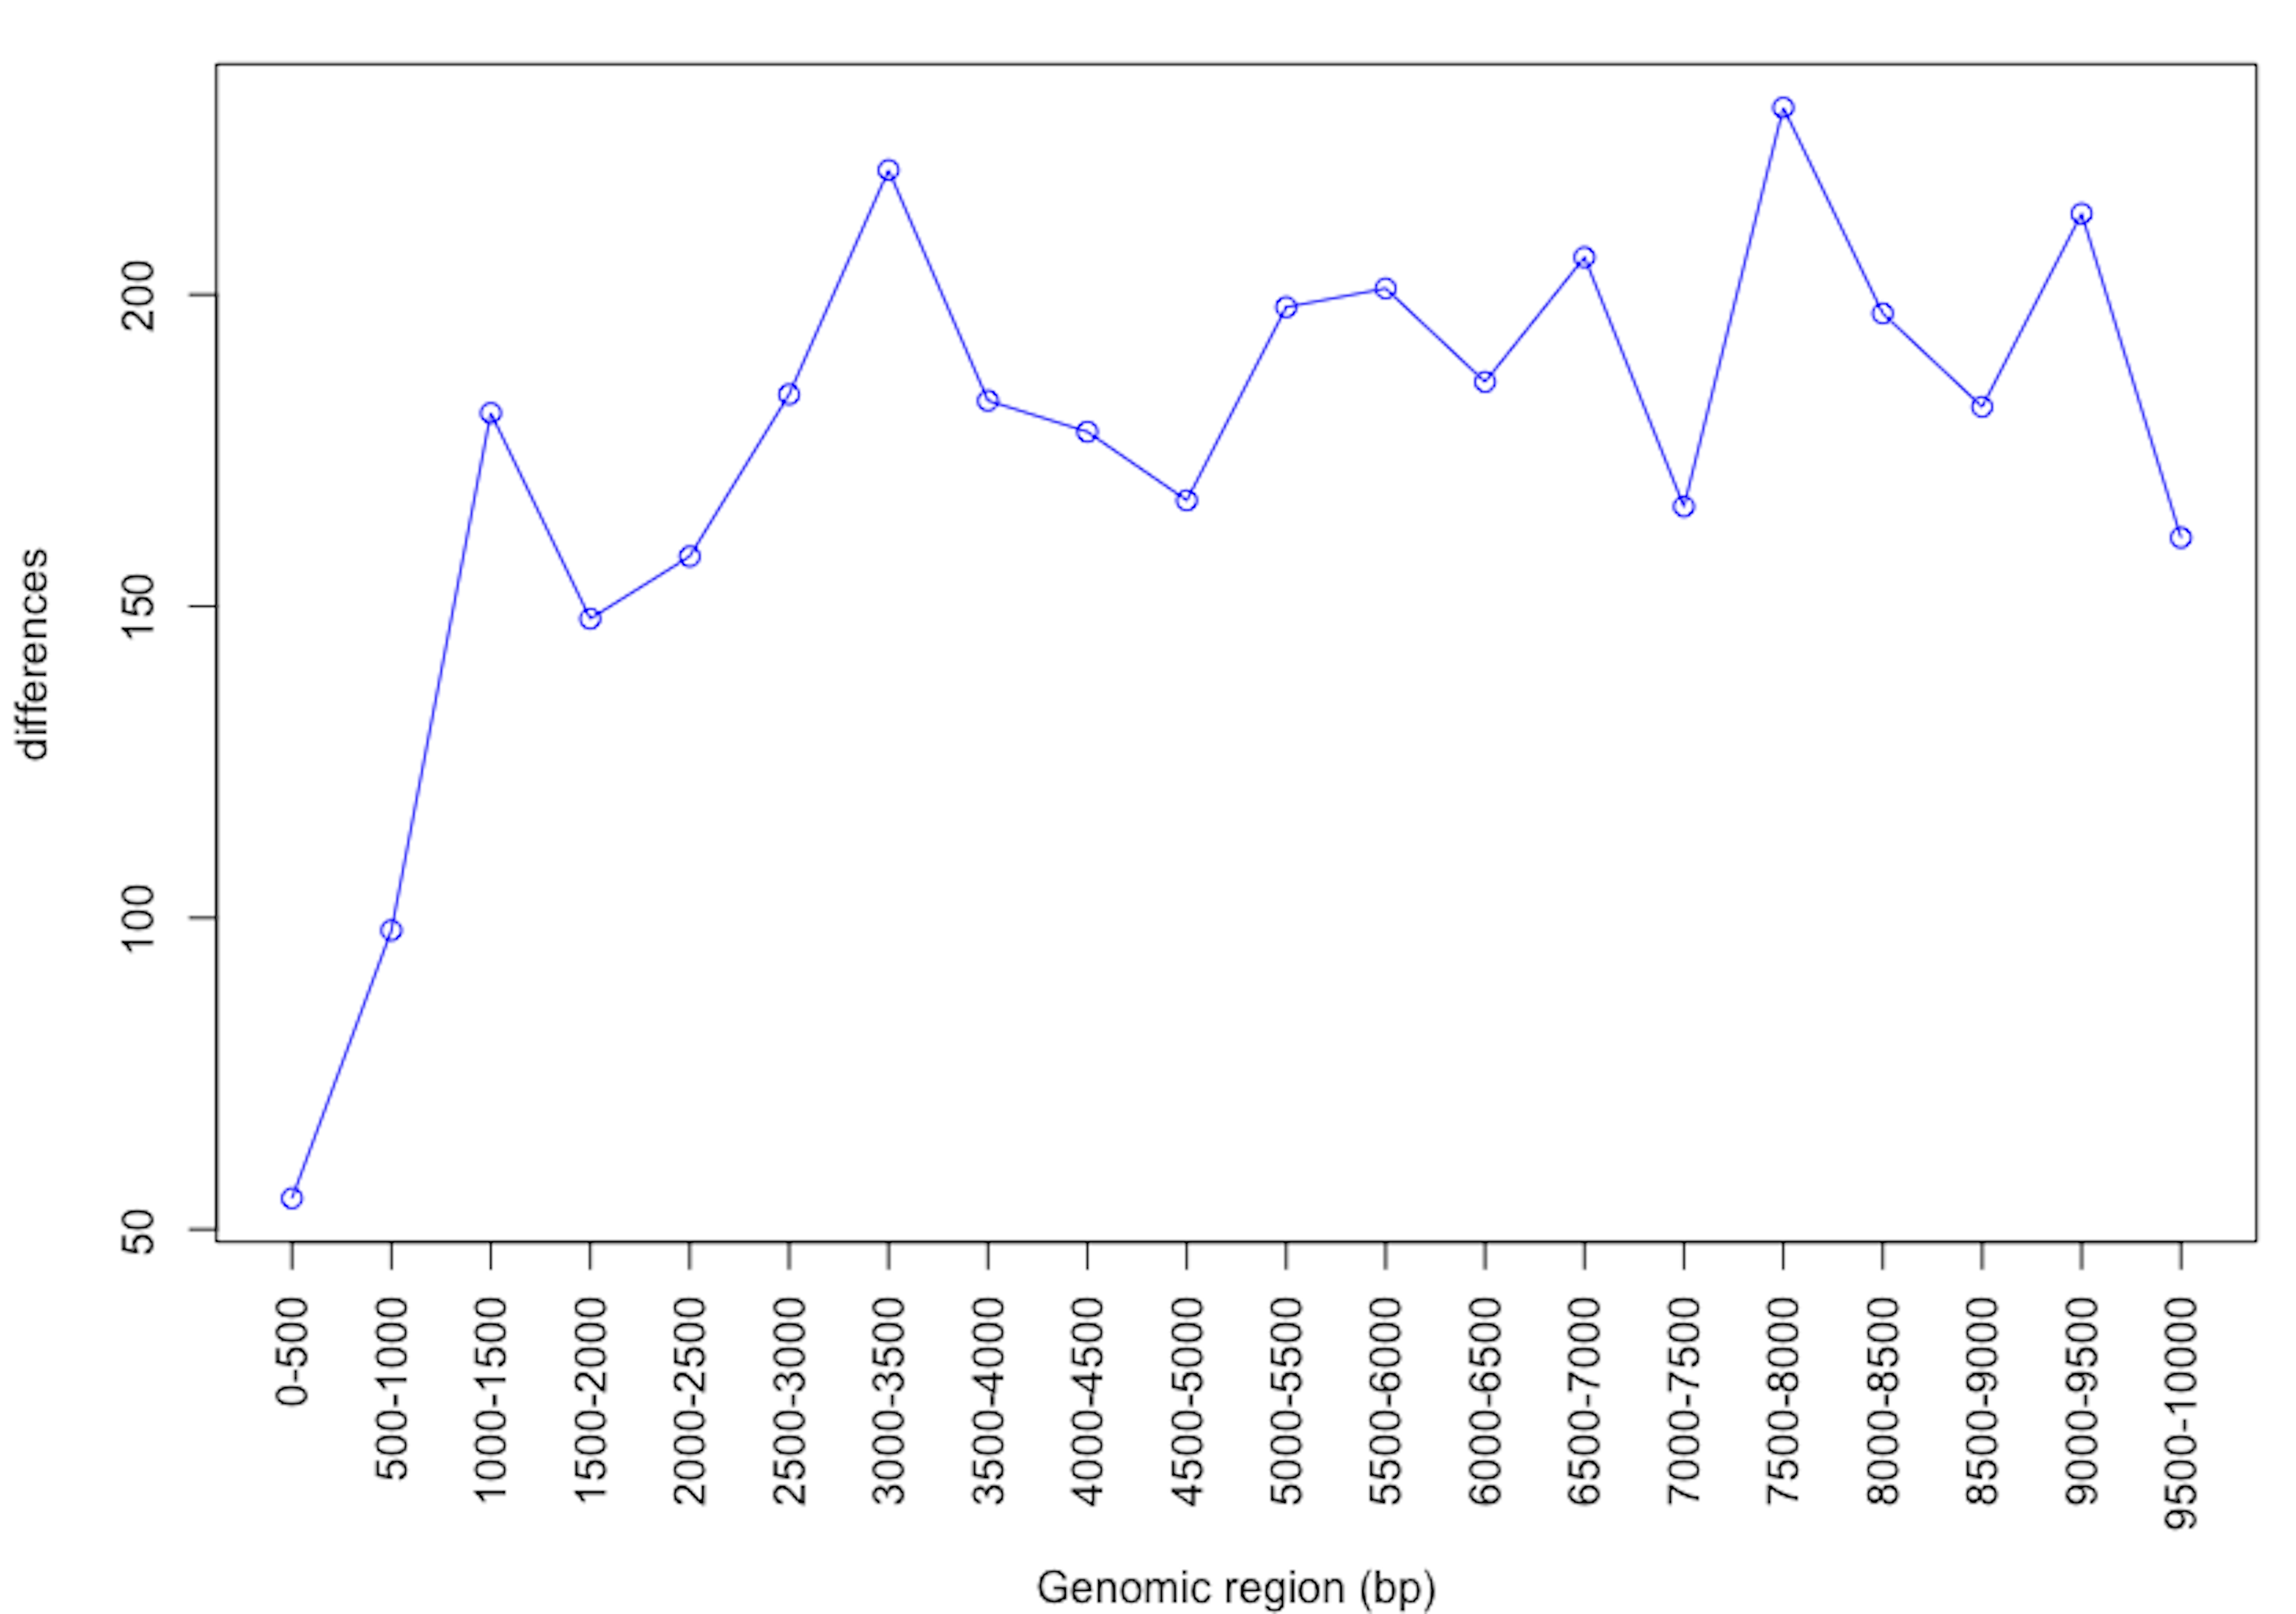
\includegraphics{figures/fig2.png}
\end{figure}

Likewise, a user may also investigate the statistical significance of specific peaks of interest at varying upstream cutoffs via the help of external software (e.g., HT-seq/edgeR, HT-seq/DESeq2, etc).  Once the user has chosen the specific upstream extension to be used, the peak file is ready to be fully annotated:

\begin{Schunk}
\begin{Sinput}
> annotate(rat, 3300)
\end{Sinput}
\end{Schunk}

which generates a fully annotated peaks file containing various genomic features and labeled headers.  

\end{document}
